\chapter{缺陷检测的深度学习方法}
\section{引言}

\section{关键技术}
CNN网络,即卷积神经网络,在图像数据上有相当优异的表现。

\subsection{卷积化}

\subsubsection{卷积的定义}

卷积是定义在两个实变函数上的一种数学运算,一般用于对数据做平滑运算。卷积操作有两个操作函数。我们以一维时间序列为例,如下面图\ref{fig:con-1D}。

有在任意t时刻的测量 $ m(t) $ ,我们以一个模板函数,或是加权函数 $ w(\tau) $

我们引入卷积运算

\begin{eqnarray}
    s(t) =  \int m(\tau)w(t-\tau)d\tau
\end{eqnarray}

而此时我们定义 $ \ast $ 为卷积操作符

平常的使用中,我们大多使用的是离散的数据,为此我们定义离散的卷积操作:

\begin{eqnarray}
    s(t) = (m \ast w)(t) = \sum^{\infty}_{\tau = -\infty} m(\tau)w(t-\tau)d\tau
\end{eqnarray}

\begin{figure}[!tbp]
    \centering
    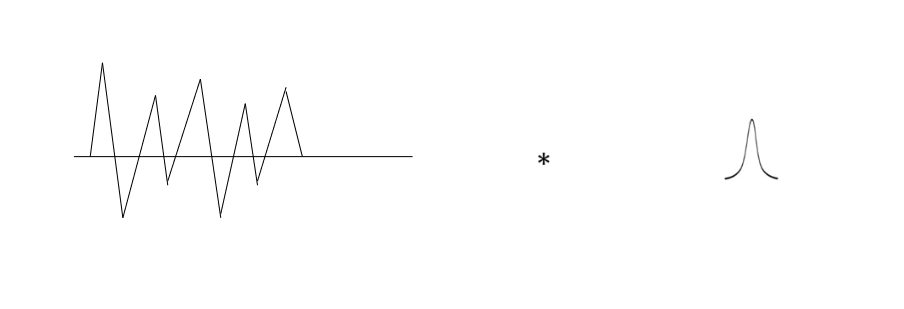
\includegraphics[width=\textwidth]{figures/con-1D.png}
    \caption{一维卷积示意图}
    \vspace{-1em}
    \label{fig:con-1D}
\end{figure}

上面的卷积操作对一维时间序列 $ m(t) $ 有了结果,最终的平滑函数s在t点的值被定义于与$ w $ 重合的模板开始的加权和上。

据此定义下的参数函数m被称为输入函数,而参数函数w被称作核函数。

计算机中使用的是离散的数据,我们通常将其放入一个数组,简单的如一维时间序列、二维的矩阵,复杂的如多维空间数组。一般的,我们称这些多维数组为张量。

图像处理中,我们通常以二维矩阵形式存储其数据结构,灰度图是单通道的,对于一个输入图I,以及我们需要的卷积核K,我们定义其卷积如下,如图\ref{fig:con-2D}:

\begin{eqnarray}
    S(i,j) = (I \ast K)(i,j) = \sum_{m} \sum_n I(m,n)K(i-m,j-n)
\end{eqnarray}

一般的,卷积核函数的尺度要远小于输入图函数的尺度,我们可以交换其位置,等价的写作:

\begin{eqnarray}
    S(i,j) = (K \ast I)(i,j) = \sum_{m} \sum_{n} I(i-m,j-n)K(m,n)
\end{eqnarray}

\begin{figure}[!tbp]
    \centering
    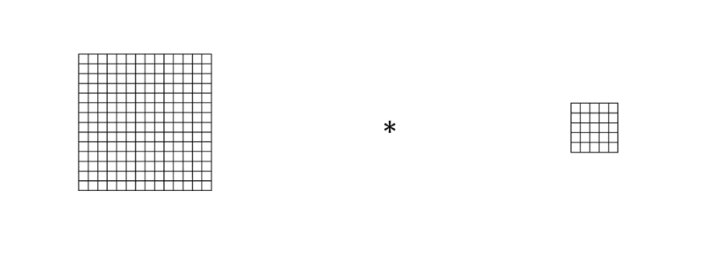
\includegraphics[width=\textwidth]{figures/con-2D.png}
    \caption{二维卷积示意图}
    \vspace{-1em}
    \label{fig:con-2D}
\end{figure}

与上面相似,最终得到了平滑后的函数图像。

%[这边可以放一张做过处理的对比图]

除开单通道的灰度图,我们还有彩色的三通道图片,为了描述其卷积效果,我们需要引入一个四维的张量核 $ K_{i,j,k,l} $ 。其中i是输出通道,j是输入通道,而k,l代表输出与输入的偏置矩阵。对于输入图像 $ I_{i,j,k} $ 即对于(j,k)位置的通道为i处的值,我们有输出S:

\begin{eqnarray}
    S_{i,j,k} = \sum_{l,m,n}I_{l,j+m,k+n}K_{i,l,m,n}
\end{eqnarray}

这里l,m,n因为在计算机中,数组一般从0计数,与普通数学计算有些许不同。

\subsubsection{卷积的意义}

在常规图像中,有大量的像素,即使在一般用于训练的小尺寸图像,也大于 $ 224 \times 224 $ 个像素,而我们对于目标的检测确只有少量特征,其中大量的参数对于我们的模型是无关的,即使需要上下文信息,但图像边缘的信息一般对于另一边缘的特征没有帮助。相比与全连接层的实现,卷积网络的稀疏连接的特点能有效减少其存储和运算需求,相比与可能存在的指数的代价,卷积网络所使用的核函数代价小得多。

其次,由于卷积网络的平滑特性,上层的节点能够感受到下层周围节点的信息,比如对于一个 $ 3 \times 3 $ 的核函数,其相对于上层单个节点能够感受到下层9个节点的信息,其有参数共享的性质。我们将其能感受到下层的区域称为感受野。
在层数增加后,顶层的节点能共享下面的极大部分区域的信息,虽然这个可能导致信息的丢失,但其能够显著地减少模型的存储需求。对于整个模型的鲁棒性也是有益的。

\subsection{池化操作}

池化函数一般接在一个卷积层的输出位置,紧接在仿射变换和线性整流后。用以对输出做进一步的处理。

池化函数的作用效果和卷积相似,都是用其位置周围的总体特征去代替网络在该位置上的输出。其最主要的作用是保持局部的平移不变性,即我们讲,即使输入的局部坐标做了少量平移,最终的输出也是几乎不变的。

\begin{figure}[!tbp]
    \centering
    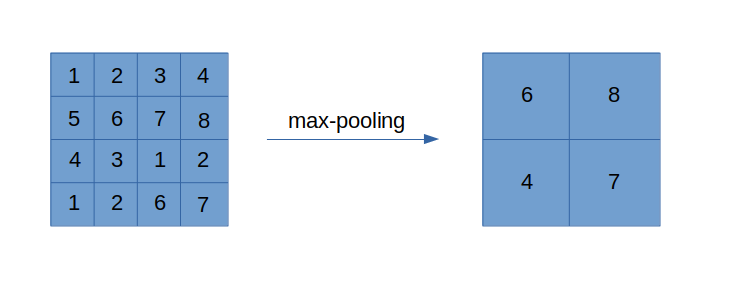
\includegraphics[width=\textwidth]{figures/max-pooling.png}
    \caption{最大池化示意图}
    \vspace{-1em}
    \label{fig:max-pooling}
\end{figure}

我们图像经常的一点就是图像的大小不一,我们图像可能拍摄出的区域并非我们需求的,一般的我们通过剪裁、平移、仿射变换等对其进行处理,但池化的引入可以让我们对不同大小的输入图像有通用的处理能力,因为池化能获得周围的总体特征,为此,下一层的输入一般可以比上一层有所减少。我们只需要调整池化层的偏置,将多余的部分转化为到有限的精简的输入特征上去,这样就能和图像大小解耦。相似的,在输出时,网络也允许有可变的大小,要是想指定数据尺寸,只需要增加池化层即可。图\ref{fig:max-pooling}就显示了最大池化。

卷积和池化均可以精简参数,但是会丢失准确的空间信息,假如有一个三层的卷积网络,其使用了 $ 3 \times 3 $ 的卷积核,那么在三层之后,所有小于3的特征是不能识别的,这也导致了可能出现的欠拟合问题。简单地,我么可以取消部分通道的池化缓解这个问题。

\subsection{空洞卷积}

另一个解决方向就是考虑空间的关系,其中最适用的就是空洞卷积理论。

为了解决卷积网络池化层的存在而导致的采样信息损失,虽然可以插值扩充整个特征表,但对于损失的信息并不能无损找回,前面简单地使用了去掉池化层以缓解这个问题,但是池化层减小会导致感受野的减小,使得局部不变性降低。而空洞卷积就是为了解决这个问题,其在空间尺度上作出了调整。

%[不确定的理论]
我们在空间尺度上即可以跳过一些位置,准确的说空洞卷积算是一种对全卷积的下采样,其中s代表步长:

\begin{eqnarray}
    S_{i,j,k} = c(K,I,s)_{i,j,k} = \sum_{l,m,n}I_{l,j \times s+m ,k \times s +n}K_{i,l,m,n}
\end{eqnarray}


同样的,对于 $ 3 \times 3 $ 的卷积核,传统卷积运算会让核和输入张量上紧凑的 $ 3 \times 3 $ 进行相乘求和,相对的,上层节点的感受野只有 $ 3 \times 3 $ 的大小。

而使用空洞卷积,卷积核会与张量中的较远的像素相乘相加,这里像素的间隔步长是稳定的。在步长为2时,感知野能够扩大到 $ 7 \times 7 $ ,步长为4时,我们能够得到 $ 15 \times 15 $ 的感知野。我们用此来替代池化层,能够保证网络的感受野不会缩小,保证了图像语义的精度。 

\begin{figure}[!tbp]
    \centering
    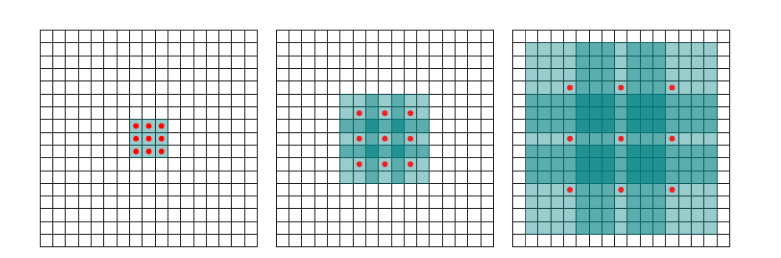
\includegraphics[width=\textwidth]{figures/dilated-convolution.png}
    \caption{空洞卷积\cite{yu2015multi}示意图}
    \vspace{-1em}
    \label{fig:dilated-convolution}
\end{figure}

\subsection{填充}

观察图\ref{fig:dilated-convolution}中卷积的图示,我们可以看到对于一个 $ k \times k $ 的卷积核 K,一般的,k为奇数,如果没有任何处理,做完卷积后,输入图I会减少 $ k - 1 $ 个像素。如果核选取的过大,我们会面对网络空间的快速缩减问题。为此,我们需要填充网络。

第一种方式就是使用零填充外围,用以保持输出的大小与输入相同,这样处理后的卷积网络规模就不会缩小,能够不断地增加卷积层数,我们称这种卷积模型为相同卷积。

但是鉴于这种卷积会在网络周围填充零元素,明显的,边缘处的像素数据会由于零元素的存在而减少其影响,导致最终的卷积输出对于边缘的表示欠佳。

为此,我们还有一种填充方法,称其为全卷积,其主要特点是让原输入中的每个像素都被访问相同的次数,要实现这一点,输出图的边界像素比中心部分输出像素使用的输入像素要更少。最终输出图宽度增加 $ k-1 $,虽然这样能有效避免边缘弱化问题,但这样核函数比较难以实现。


\section{基于深度学习的检测模型}

\subsection{前馈神经网络}
深度网络最基本的就是深度前馈网络,或者称其为多层感知机,图\ref{fig:alex-net}中显示了alexnet的网络结构。

\begin{figure}[!tbp]
    \centering
    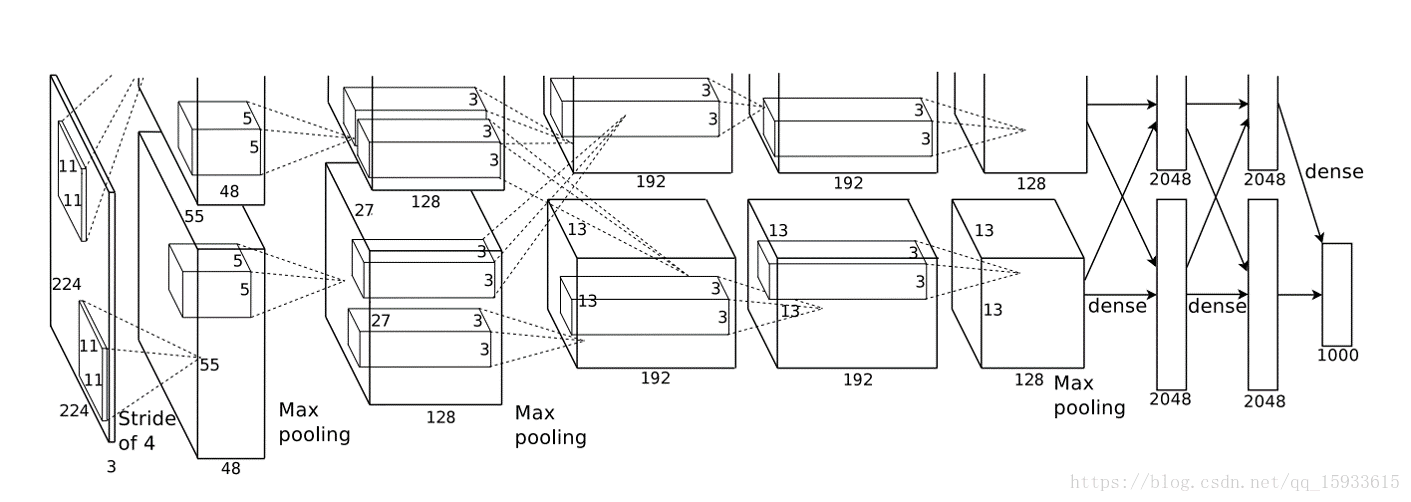
\includegraphics[width=\textwidth]{figures/alex-net.png}
    \caption{alex-net的网络结构\cite{NIPS2012_4824}}
    \vspace{-1em}
    \label{fig:alex-net}
\end{figure}

前馈网络的前向性体现在输出与输入之间的信息传递是单向的,输入数据x,仅在经历了数个仿射变换和函数映射后单项转化为输出y。

在前馈网络中,数个映射 $ f^{(i)} $ 形成函数链:

\begin{eqnarray}
    y = f(x) = f^{(n)}(\cdots f^{(3)}(f^{(2)}(f^{(1)}(x))))
\end{eqnarray}

此处n我们定义为前馈网络的深度,或是称其为层数,x称为输入层,y称为输出层,i称为这个前馈网络的层数。

但在实际运用中我们并非能够得到我们的真实映射函数 $ f(x) $ ,我们一般只能得到一些映射函数的近似函数 $ f^{\ast}(x) $ ,显然最终的结果 $ y^{\ast} $ 与真实值有所差距 $ y $ ,为了减少这个差距,提升精度,我们需要学习这个近似函数 $ y^{\ast} $ 的最好表达。

类似于神经结构,我们中间有很多函数是无法直接对我们的输出产生直接的影响,而我们采集的数据并不可能对中间层的输出有联系,因此这些对于我们的外围接口来说是一个近似黑盒的结构,其中的过程是对接口隐藏的,我们将其称为隐藏层。

隐藏层的增加是很有用的,层数的增加能让上层节点感受到更多更复杂的下层节点信息,能有效增加训练结果的精确性。

\subsection{激活函数}

隐藏层的引入意味着我们需要一个隐藏层的激活函数,一般的,下层到上层的变换是通过一个仿射变换实现的。

简单的我们以线性回归定义:

\begin{eqnarray}
    h = g(W^Tx+b)
\end{eqnarray}
 
其中h代表了单个隐藏层的输出,x是输入,W是我们做仿射变换的矩阵,b是变换的偏置。而g是激活函数。

激活函数一般使用了一个非线性函数以实现网络额参数控制,如果缺失了这个函数,我们的网络实际就由多个线性函数叠加实现,导致最后的网络仍是线性的。

而ReLU函数或称为整流线性单元是我们最常使用的激活函数,其是取到输出和0相比的较大值,即我们写作:

\begin{eqnarray}
    g(y) = \max \lbrace 0,y \rbrace
\end{eqnarray}

\subsection{代价函数}

我们刚才提到了我们的由近似映射 $ f^{\ast} $ 和 真实映射 $ f $ 会分别产生近似输出 $ y^{\ast} $ 和真实输出 $ y $ ,一般的,其中真实输出就是我们的检测的输入数据的分类或是标签,其中会有相当的误差 $ y^{\ast} - y $。我们的目标是最小化误差。

为此我们引入了代价函数J,代价函数是对误差的代价分析,代价函数的选取适宜能有效减少训练的时间和成本。

最大似然是常使用的一种代价函数,其表示为概率分布的负对数,香农的信息论中使用这个来表示我们的估计概率分布中真实事件的发生概率,交叉熵损失函数用以衡量我们的估计分布和真实分布的相似性:

\begin{eqnarray}
    J(\Theta) = - E_{x,y \sim \hat{p}}logP^{\ast}(y|x)
\end{eqnarray}

上面 $ \hat{p} $ 代表数据的真实分布,$ p^{\ast} $ 代表我们的估计分布。

当然代价函数也是随着模型的变化而变化的,我们还有许多其他的代价函数。

代价函数在设计时还有些注意的事项:深度前馈网络很大程度上是通过梯度下降实现的,因此其需要有很大的梯度,防止因为梯度太小而导致的无法优化问题,在这问题上,均方误差和平均绝对误差就成效不佳。因此,足够的预测性能够指明我们的学习方向。


\subsection{反向传播}

在深度神经网络中,信息的流动一般是前向的,输入 $ x $ 后信息会通过网络的节点流动,最终传到最终输出 $ y^{\ast} $ ,就是信息的前向传播。一般的,我们要优化中间各层的权重,即我们需要输出处的信息反向流回输入,以此来计算梯度。

我们考虑标量情况,对于从 $ R^{m} $ 到 $ R^{n} $ 的映射 $ y=g(x) $ 和从 $ R^{n} $ 到 $ R $ 的映射 $ z=f(y) $ 来说,我们可以运用链式法则:

\begin{eqnarray}
    \frac{\partial z}{\partial x_i} = \sum_{j} \frac{\partial z}{\partial y_j} \frac{\partial y_j}{\partial x_i}
\end{eqnarray}

即我们表示为:

\begin{eqnarray}
    \nabla_x z = (\frac{\partial y}{\partial x})^T \nabla_y z
\end{eqnarray} 

明显的,张量$ \mathtt{X} $也能以类似的表示方法来看,虽然其可能有多个维度,或者多个坐标进行索引,但是在计算机中我们完全可以将其扁平化,使用一个主键进行索引,与上面相似的:

\begin{eqnarray}
    \nabla_{\mathtt{X}}z = \sum_{j}(\nabla_{\mathtt{X}}Y_j)\frac{\partial z}{\partial \mathtt{Y}_j}
\end{eqnarray}

这就是反向传播算法的基础,当整个是由多个节点级联而成的时候,反向传播算法会对每一个节点执行一次雅可比乘积,并以此通过链式法则得到最后针对于输入的梯度实现。

对于反向传播算法,其在计算了输出单元的误差之后会反向及计算所有上一层到下一层的权值并以此更新权重,这也是我们一般意义上的梯度下降法。

\section{数据集介绍}
我们使用了dagm2007表面缺陷图像数据作为我们的数据源,dagm2007是第29届德国模式识别协会年度研讨会的评价数据集,由欧洲神经网络学会(GNNS)的德国分会提供。其包含了10类共8000张图像,并提供了大量正负样本和标签。并分成了训练集和测试集。

\section{本章总结}
本章对缺陷检测的深度学习方法进行了介绍,介绍了在深度学习的卷积神经网络中需要的基础知识,如卷积的定义、降采样、池化,以及网络的运行和训练原理,涉及到反向传播的定义和使用,以及网络的优化方法,即损失函数的定义和设置。以及相关改进,比如如何降低网络的计算量和提升精度。
